\chapter{Accept user input}

\section{Video: What is the TextInput component?}
\subsection{Use case in this project}
\begin{itemize}
    \item Little Lemon App want to get the feedback from the customer.
    \item They allow users to type in their name, contact details and custom messages.
\end{itemize}

\subsection{TextInput}
\begin{itemize}
    \item A native component that will open up the native iOS or Android keyboard depending on the device you are using.
    \item The same code, users have different experiences across platform.
    \item Benefits:
    \begin{itemize}
        \item Auto correction
        \item Placeholder text
        \item Support for different keyboard types
        \item Auto capitalization
    \end{itemize}
\end{itemize}

\subsection{Syntax}
\begin{itemize}
    \item TextInput syntax
\end{itemize}
\begin{lstlisting}[language=Java, numbers=none]
    <TextInput
        // Styles
        style={styles.input}
        onChangeText={onChangeFirstName}
        // Default text in input box
        placeholder='First name'
        // Value displayed in the input box
        value={firstName}
    />
\end{lstlisting}
\begin{itemize}
    \item \texttt{onChangeText}
    \begin{itemize}
        \item Its a callback.
        \item Use with \texttt{useState()}
        \begin{lstlisting}[language=Java, numbers=none]
            const [firstName, onChangeFirstName] = useState('')
        \end{lstlisting}
    \end{itemize}
    
    \item \textbf{Practice Question:} In the Little Lemon mobile app, you’d like a to add a text input box that displays the text “Email address” before the user types anything inside of it. Which prop would you pass in to accomplish this?
    $\rightarrow$ placeholder 
\end{itemize}

\begin{itemize}
    \item More props:
    \begin{itemize}
        \item \texttt{keyboardType}: "default","number pad", "decimal pad", "numeric", "email address", "phone pad", ...
    \end{itemize}
\end{itemize}

\section{Video: Configure the TextInput Component}
\begin{itemize}
    \item \textbf{Practice Question:} You are adding a text input box to your app for the user to enter their email address. You will need to configure at least two separate \texttt{TextInput} components to do this – one for iOS devices, and another for Android devices. True or false?  
    $\rightarrow$ False 
\end{itemize}

\section{Reading: TextInput Component and its Feature}
\begin{figure}[H]
    \centering
    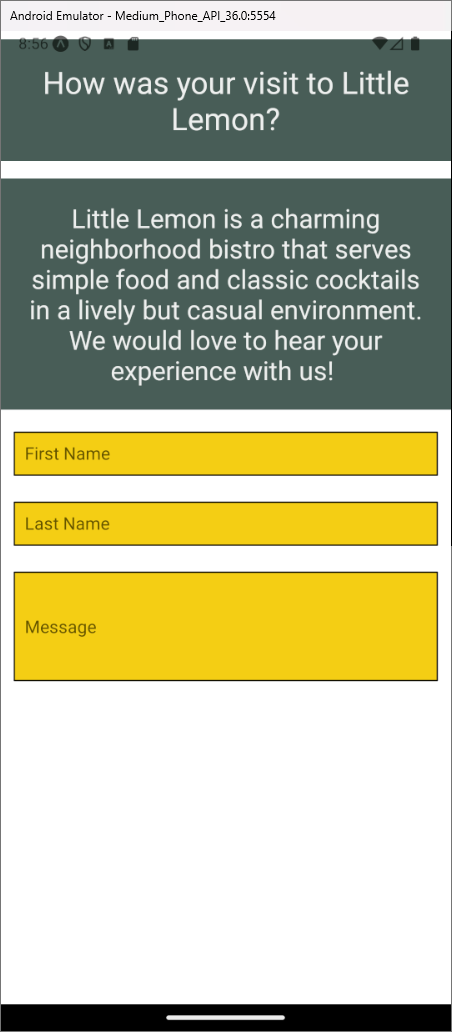
\includegraphics[width=0.2\textwidth]{images/ex4.png}
    \caption{TextInput Component}
\end{figure}

\section{Reading: Exercise: Create a TextInput Component}
\begin{figure}[H]
    \centering
    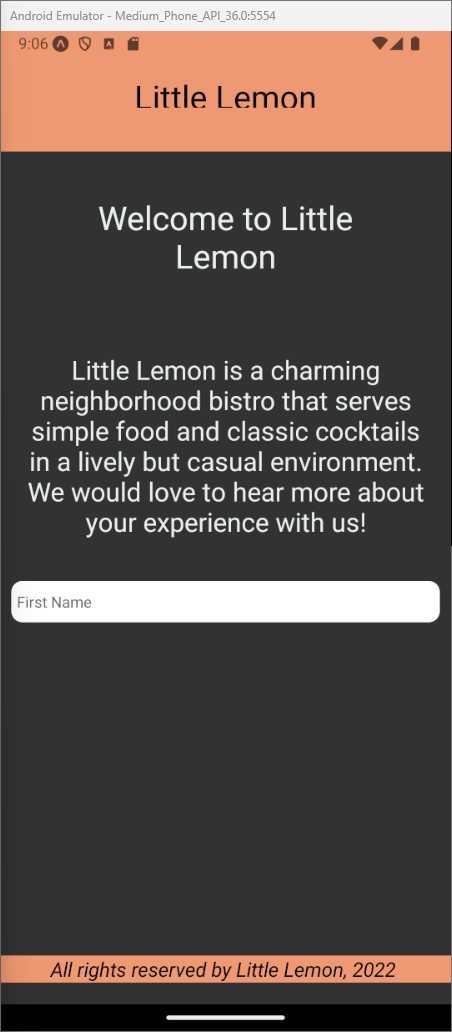
\includegraphics[width=0.2\textwidth]{images/Ex4 (2).png}
    \caption{Exercise: Create a TextInput Component}
\end{figure}

\section{Practice Assignment: Self review: Create a TextInput Component}
\begin{figure}[H]
    \centering
    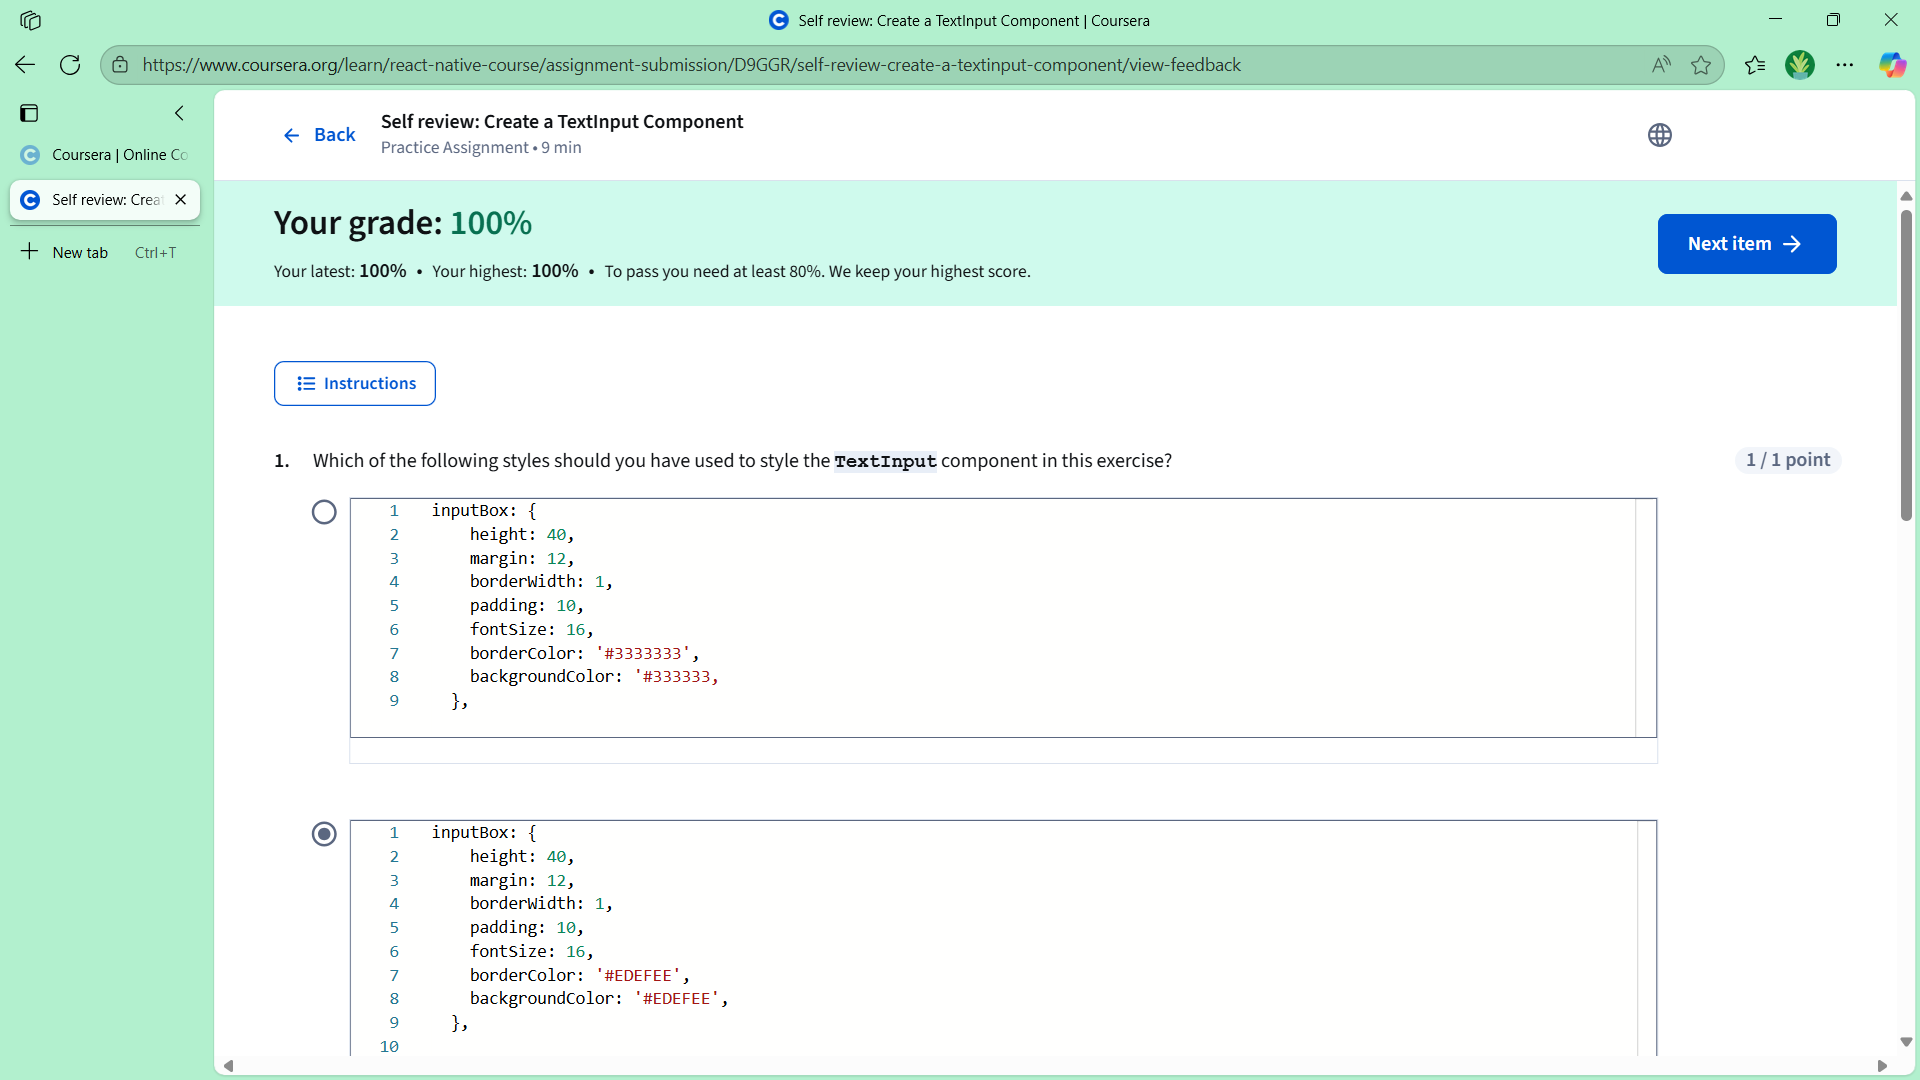
\includegraphics[width=0.5\textwidth]{images/sr-3.png}
    \caption{Self review: Create a TextInput Component}
\end{figure}

\section{Video: Virtual Keyboard on Mobiles App}
\subsection{Problem about keyboard}
\begin{itemize}
    \item Open the virtual keyboard in an emulator:
    \item Ctrl/Cmd + Shift + K
    \item When the keyboard opens, it may cover important parts of your app. 
\end{itemize}

\subsection{React Native Props}
\begin{itemize}
    \item \texttt{keyboardDismissMode} property
    \begin{itemize}
        \item The keyboard will be dismissed when user scrolls the view.
        \begin{lstlisting}[language=Java, numbers=none]
            <ScrollView keyboardDismissMode='on-drag'/>
        \end{lstlisting}
        \item Set to none if you want the keyboard to stay open even when the user scrolls the view.
    \end{itemize}

    \item \texttt{KeyboardAvoidingView} component
    \begin{itemize}
        \item Automatically adjust its height, position, or padding to avoid conflict with other views.
        \item Push the view on the top of the keyboard when it appears.
        \item This component inherit all the props of the View component.
        \begin{lstlisting}[language=Java, numbers=none]
            <KeyboardAvoidingView
                behavior={Platform.OS === 'ios' ? 'padding' : 'position'}
            >
                <TextInput
                    style={styles.input}
                    onChangeText={onChangeFirstName}
                    placeholder='First name'
                    value={firstName}
                />
            </KeyboardAvoidingView>
        \end{lstlisting}
    \end{itemize}

    \item \textbf{Practice Question:} Your app has text input boxes that open the virtual keyboard when tapped. For the \texttt{keyboardDismissMode} property of the \texttt{ScrollView}, you’ve set the value to \texttt{on-drag}. What does this do?   
    $\rightarrow$ The virtual keyboard will be dismissed when the user scrolls.   
\end{itemize}

\section{Reading: Tips and Tricks to handle virtual keyboard}
This part is the same as in the previous section about virtual keyboard.

\section{Video: Handling the Virtual Keyboard}
\begin{itemize}
    \item \textbf{Practice Question:} In your mobile app, you want to set the virtual keyboard to be dismissed as soon as the user scrolls. Which value of \texttt{keyboardDismissMode} would you assign to set this behavior?   
    $\rightarrow$ on-drag
\end{itemize}

\section{Practice Assignment: Knowledge Check: Accept user input}
\begin{figure}[H]
    \centering
    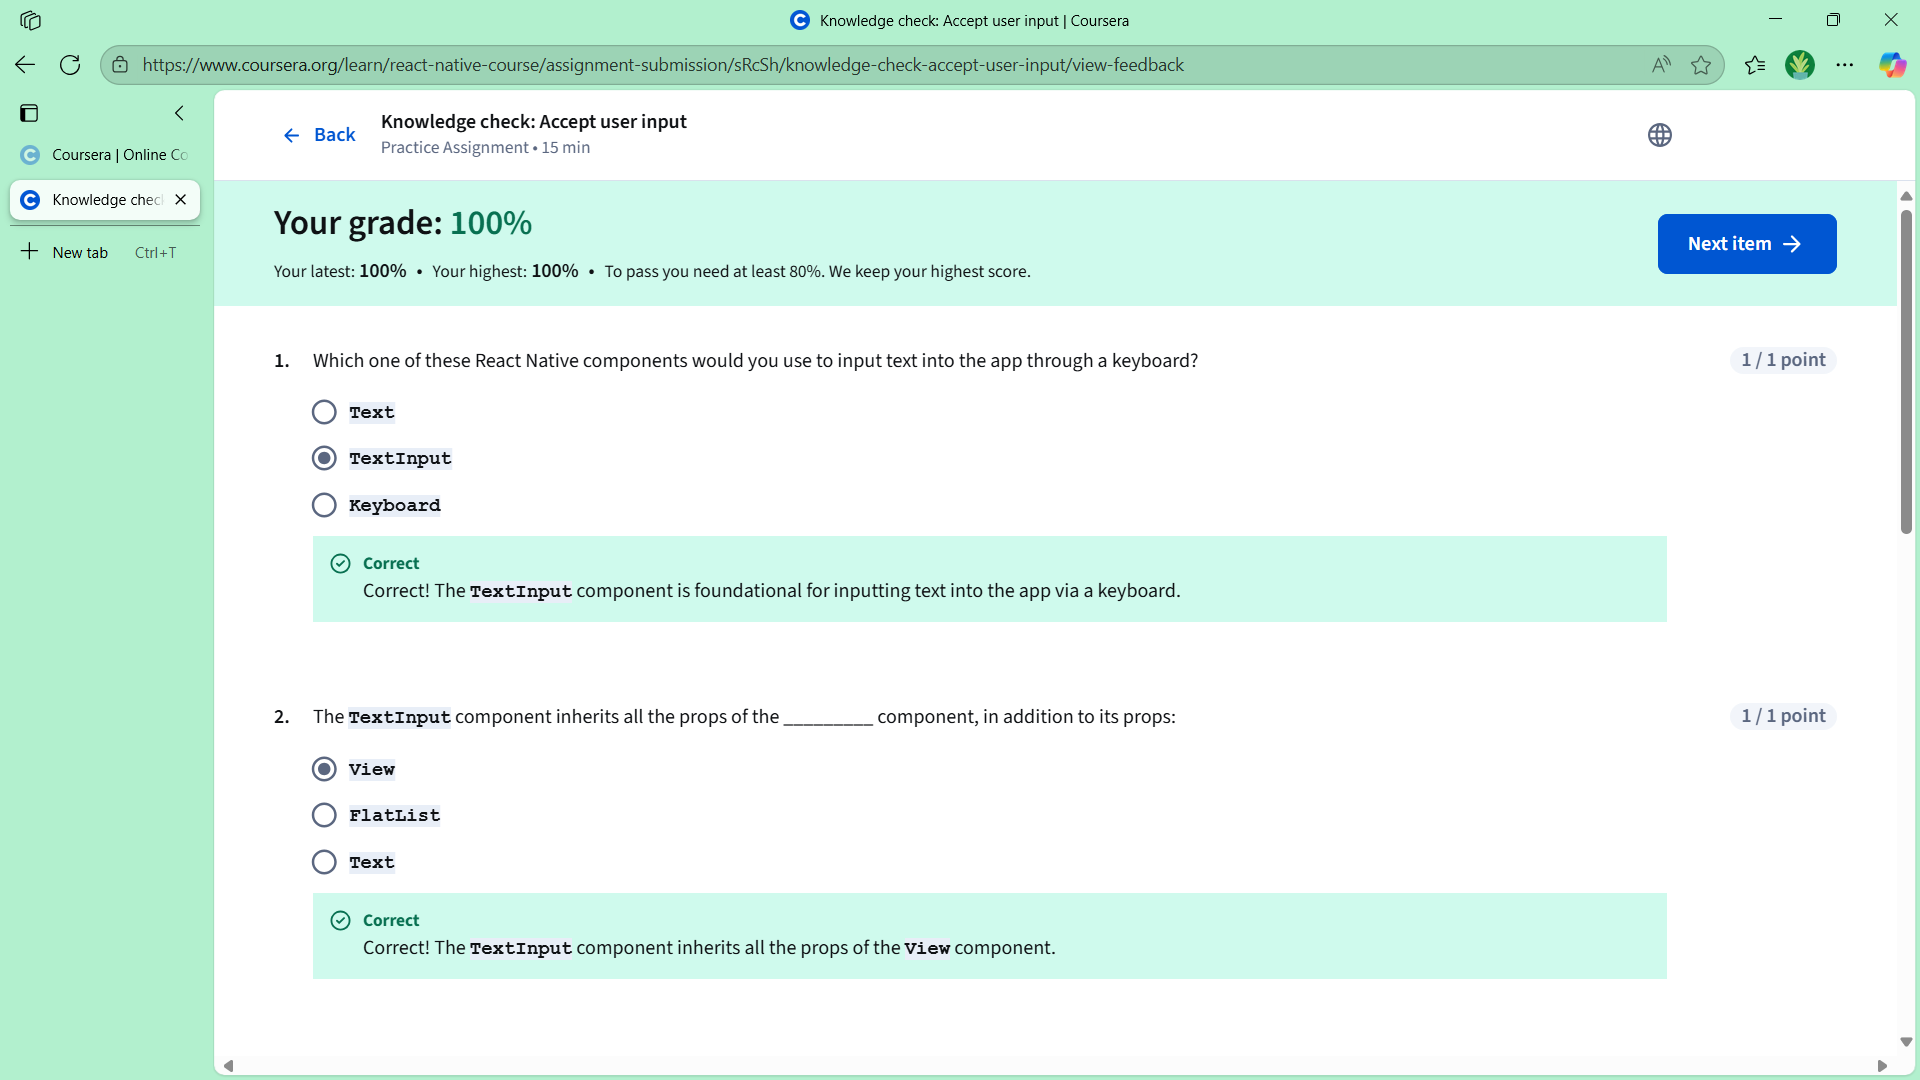
\includegraphics[width=0.5\textwidth]{images/kc-3.png}
    \caption{Knowledge Check: Accept user input}
\end{figure}